% =====================================================================
%  Comparative review: groundwater of the Suketi basin and Gaj watershed,
%  Himachal Pradesh. Single column, numbered sections, author--year
%  citations (natbib). Compile: pdflatex main.tex (run twice).
% =====================================================================
\documentclass[11pt,a4paper]{article}

% ---------------- Author details (edit before submission) -------------
\newcommand{\Authors}{Author Name\textsuperscript{1*} and Author Name\textsuperscript{2}}
\newcommand{\Affiliations}{%
  \textsuperscript{1}Department, Institution, City -- PIN, India\\
  \textsuperscript{2}Department, Institution, City -- PIN, India\\
  \textsuperscript{*}Corresponding author: email@example.com}

% ---------------- Packages -------------------------------------------
\usepackage[T1]{fontenc}
\usepackage[utf8]{inputenc}
\usepackage{mathptmx}
\usepackage[a4paper,margin=2.3cm]{geometry}
\usepackage{amsmath}
\usepackage[version=4]{mhchem}
\usepackage{booktabs,tabularx,array}
\usepackage[font=small,labelfont=bf,labelsep=period,skip=4pt]{caption}
\usepackage{titlesec}
\usepackage[round,authoryear]{natbib}
\usepackage{xcolor}
\usepackage{pgfplots}
\pgfplotsset{compat=1.16}
\usepackage{enumitem}
\usepackage{microtype}
\usepackage{xurl}
\usepackage[colorlinks=true,linkcolor=black,citecolor=black,urlcolor=blue]{hyperref}
\urlstyle{same}

\titleformat{\section}{\large\bfseries}{\thesection.}{0.6em}{}
\titleformat{\subsection}{\normalsize\bfseries}{\thesubsection}{0.6em}{}
\titlespacing*{\section}{0pt}{12pt plus 2pt}{5pt}
\titlespacing*{\subsection}{0pt}{9pt plus 2pt}{3pt}
\setlist{itemsep=2pt,topsep=3pt}
\renewcommand{\topfraction}{0.85}
\renewcommand{\textfraction}{0.1}
\renewcommand{\floatpagefraction}{0.75}
\renewcommand{\arraystretch}{1.2}
\newcolumntype{L}{>{\raggedright\arraybackslash}X}
\definecolor{barA}{RGB}{70,110,160}
\definecolor{barB}{RGB}{214,140,60}

\newcommand{\kmsq}{km\textsuperscript{2}}
\newcommand{\Mm}{Mm\textsuperscript{3}}
\newcommand{\uScm}{$\mu$S/cm}

% =====================================================================
\begin{document}

\begin{center}
{\Large\bfseries Groundwater Occurrence, Hydrochemistry and Recharge Planning in Two
Himalayan Catchments of Himachal Pradesh, India: A Comparative Review of the Suketi
Basin and the Gaj Watershed\par}
\vspace{1em}
{\normalsize \Authors\par}
\vspace{0.4em}
{\small\itshape \Affiliations\par}
\end{center}

\vspace{0.6em}
\hrule
\vspace{0.6em}
\noindent\textbf{Abstract}\par\vspace{0.3em}
\noindent
Groundwater planning in the Himalaya has to deal with steep slopes, fault-controlled
aquifers, a short monsoon and growing demand. This review compares three studies from
Himachal Pradesh, India. Two of them deal with the Suketi river basin in Mandi district: one
describes its groundwater resource and development needs, and the other reports the
chemistry of its groundwater in May and November 2009. The third maps groundwater potential
in the Gaj watershed of Kangra district for 2010 and 2022 using GIS and the analytic hierarchy
process, and proposes sites for recharge structures. In the Suketi basin, the alluvium of the
Balh valley holds most of the usable groundwater, and only about 22\% of the assessed
resource is in use. The surrounding hills depend on small springs, many of which almost stop
flowing before the monsoon. The water is mainly of Ca--HCO\textsubscript{3} type and is
suitable for drinking and irrigation, except for fluoride of 4.2~mg/L in one bore well on
granite and nitrate of 28--37~mg/L at two town sites. In the Gaj watershed, the area of very
high potential became smaller between 2010 and 2022 as monsoon rainfall declined, and the
recommended recharge sites lie on low to moderate slopes near settlements. The studies treat
quantity, quality and site selection separately. We identify the main gaps in data and method
and suggest how future work can link these three parts.

\vspace{0.5em}
\noindent\textbf{Keywords:} Himalayan hydrogeology; Springs; Water quality; Groundwater
potential; Analytic hierarchy process; Artificial recharge.
\vspace{0.6em}
\hrule
\vspace{0.8em}

% =====================================================================
\section{Introduction}

Groundwater meets a large part of India's drinking and irrigation needs, and satellite data
show that storage has been falling in many northern states \citep{rodell2009}. In mountain
regions, groundwater also keeps streams flowing in the dry season and feeds the springs on
which many villages depend \citep{somers2020}. In the Indian Himalaya, falling spring discharge
has been reported for several decades \citep{valdiya1989}, and a national working group has
called for a systematic effort to map and revive springs \citep{niti2018}.

Hill aquifers are hard to study. Slopes are steep, so much of the rain runs off before it can
soak in. Thrusts and fractures break the rock into small, poorly connected aquifers. Field
data are scarce, and in Himachal Pradesh official groundwater estimates are prepared only for
valley areas \citep{cgwb2006}. Meanwhile, population, tourism and farming are growing in the
foothill districts of Mandi and Kangra.

A sound management plan needs three kinds of information: how much groundwater there is
and where, whether it is safe to use, and where recharge structures should be built. Three
studies from the Beas catchment each provide one of these:
\begin{enumerate}
  \item \citet{pophare2015} described groundwater occurrence, wells, springs and
        management options in the Suketi river basin.
  \item \citet{pophare2018} studied the chemistry and quality of groundwater in the same
        basin.
  \item \citet{sharma2025} mapped groundwater potential in the Gaj watershed using remote
        sensing, GIS and multi-criteria analysis, and selected sites for artificial recharge.
\end{enumerate}

This review compares these studies, brings their main results together and points out what
is still missing. Each paper was read in full, and its setting, data, methods, results and
recommendations were noted. Values that we calculated from the published data are marked as
derived.

% =====================================================================
\section{Geological and Physiographic Setting}

Both catchments drain to the Beas river and lie in the Lesser and Outer (Sub-) Himalaya of
Himachal Pradesh. Their main features are listed in Table~\ref{tab:setting}.

\begin{table}[htbp]
\centering
\caption{Physical setting of the two catchments.}
\label{tab:setting}
\small
\begin{tabularx}{\textwidth}{@{}p{3.0cm}LL@{}}
\toprule
\textbf{Feature} & \textbf{Suketi river basin} & \textbf{Gaj watershed}\\
& \citep{pophare2015,pophare2018} & \citep{sharma2025}\\
\midrule
District & Mandi & Kangra\\
Area & 422~\kmsq{} (Balh valley 79~\kmsq{}; hills 343~\kmsq{}) & About 900~\kmsq{}\\
Elevation & 760--2,890~m & Foothills to about 4,550~m\\
Rainfall & About 1,136~mm/yr, mainly July--September & About 2,600~mm/yr, mainly monsoon\\
Main thrusts & Mandi thrust and Main Central Thrust & Main Boundary Thrust; Jawalamukhi, Drini, Panjal and Chail thrusts\\
Porous aquifer & Quaternary fill of the Balh valley, up to about 370~m thick & Alluvium in the south; Siwalik sandstones and conglomerates\\
Hard-rock aquifer & Meta-sediments, Dhauladhar granite, Shali limestone, Subathu and Siwalik rocks & Chail formation, Dhauladhar granite\\
\bottomrule
\end{tabularx}
\end{table}

The Suketi basin has a sharp contrast in landform. In its centre lies the Balh valley, a flat
intermontane basin near 790~m, filled with boulders, gravel, sand and clay. It is enclosed by
hills that rise to almost 2,900~m and are made of older meta-sedimentary rocks, granite and
limestone \citep{srikantia1998}. The valley lies between the Mandi thrust and the Main Central
Thrust.

The Gaj watershed is larger, higher and much wetter. It drains the southern side of the
Dhauladhar range. Its upper part is made of granite and metamorphic rocks cut by thrust
faults, while the lower part has Siwalik sediments and alluvium. The area is seismically
active \citep{kumar2001}, and most of its springs lie along faults and thrusts
\citep{sharma2025}.

In short, both catchments combine one porous aquifer with good storage and a much larger
area of fractured hard rock with little storage.

% =====================================================================
\section{Methods Used in the Three Studies}

\begin{itemize}
  \item \textbf{Field hydrogeology.} \citet{pophare2015} measured the water level in 28 dug
        wells in May and November 2009, compiled records of 64 tube wells, and visited 93
        springs, which they classed by discharge after \citet{meinzer1923}. They also prepared
        maps of geology, drainage, soil, land use, lineaments and slope, and divided the basin
        into 53 small watersheds for planning. Drainage analysis gave a drainage density of
        2.69~km/\kmsq{} and an infiltration number of 10.66 \citep{pophare2014}.
  \item \textbf{Hydrochemistry.} \citet{pophare2018} sampled 31 groundwater sources (dug
        wells, tube wells, springs and bore wells) and five river sites in both seasons of
        2009. Fourteen parameters were measured by standard methods \citep{apha1998}. The
        results were read with Piper and Gibbs diagrams \citep{piper1944,gibbs1970} and with
        irrigation indices such as the sodium adsorption ratio (SAR), percent sodium and
        residual sodium carbonate (RSC) \citep{richards1954}.
  \item \textbf{GIS and multi-criteria analysis.} \citet{sharma2025} prepared eleven map
        layers from a 12.5~m ALOS PALSAR elevation model, LISS-IV satellite imagery, FAO soil
        data and rainfall and temperature records. Strongly related layers were removed with
        the variance inflation factor, weights were assigned with the analytic hierarchy
        process \citep{saaty1980}, and the layers were combined by weighted overlay. Four maps
        were made (before and after the monsoon in 2010 and 2022) by changing only the rainfall
        layer. The maps were checked with the area under the ROC curve.
\end{itemize}

% =====================================================================
\section{Groundwater Occurrence and Storage}

\subsection{Valley and hill aquifers}

The two settings behave very differently (Table~\ref{tab:regimes}).

\begin{table}[htbp]
\centering
\caption{Groundwater in the Balh valley and in the hills of the Suketi basin \citep{pophare2015}.}
\label{tab:regimes}
\small
\begin{tabularx}{\textwidth}{@{}p{3.0cm}LL@{}}
\toprule
\textbf{Parameter} & \textbf{Balh valley} & \textbf{Hills}\\
\midrule
Aquifer & Layered Quaternary gravel, sand and clay & Weathered and fractured sandstone, phyllite, granite, limestone\\
Main sources & Dug wells (up to 15~m); tube wells (mostly 50--125~m) & Springs; hand-pump bore wells (50--70~m)\\
Depth to water (2009) & Less than 12~m in May; less than 10~m in November & Not measured; many springs dry or nearly dry in May\\
Seasonal change & Less than 2~m in 27 of 28 wells & Spring flow rises after the monsoon, then falls quickly\\
Yield & Tube wells mostly 9--45~L/s; some flow at the surface & Most springs below 1~L/s (Meinzer classes VI--VIII)\\
Use of resource & About 22\% of net availability (3.48~\Mm{}/yr) & Not assessed officially\\
\bottomrule
\end{tabularx}
\end{table}

In the Balh valley, the water table lies within 4~m of the surface in more than half of the
observation wells. The net annual availability is about 3.48~\Mm{}, against a draft of only
0.78~\Mm{}, so about 2.46~\Mm{} a year remains available for future use \citep{cgwb2006}. Some
deep tube wells flow at the surface without pumping. Where the water table is within 2~m of the
surface, there is a risk of waterlogging \citep{pophare2015}.

The hills are much poorer. Of the 93 springs studied, most are fracture or depression springs.
In May 2009 many were dry or gave less than 0.01~L/s, and in November most gave only
0.1--0.4~L/s. A few springs on limestone or major faults, near Nalni, Nagchalla and Mandi, gave
more than 10~L/s. The fine drainage texture and high infiltration number show that rain leaves
the slopes quickly \citep{pophare2014}. The authors recognised three slope belts: slopes above
10\textdegree{} that mainly shed water, a 5--10\textdegree{} foot-hill belt that is the main
recharge zone, and the valley floor below 5\textdegree{} where groundwater comes out.

In the Kangra district, records quoted by \citet{sharma2025} show water-level falls of up to
7.16~m and a decadal change of about 6~m. Of 4,535 hand pumps in the area, 235 needed repair or
replacement, partly because of low water levels at some sites.

\subsection{Change in groundwater potential, 2010--2022}

In the Gaj watershed, the zones of moderate to very high potential follow the main thrusts and
lineaments and the southern alluvium \citep{sharma2025}. Between 2010 and 2022, the very high
class fell from 4.20\% to 2.63\% of the area before the monsoon, and from 4.46\% to 3.20\% after
it (Fig.~\ref{fig:gwp}). Monsoon rainfall was lower in several of the later years. The maps gave
AUC values of 0.82 and 0.81, which is normally taken as good accuracy.

\begin{figure}[htbp]
\centering
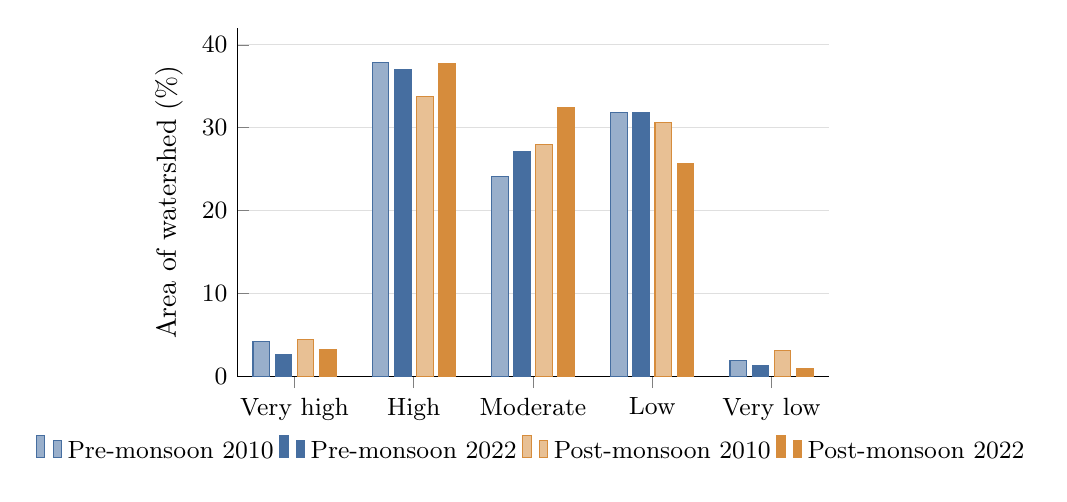
\begin{tikzpicture}
\begin{axis}[
  width=0.75\textwidth, height=6cm,
  ybar, bar width=6pt,
  ymin=0, ymax=42,
  ylabel={Area of watershed (\%)},
  symbolic x coords={Very high,High,Moderate,Low,Very low},
  xtick=data, tick label style={font=\small},
  legend style={font=\small,at={(0.5,-0.15)},anchor=north,legend columns=4,draw=none},
  enlarge x limits=0.12,
  axis lines*=left, ymajorgrids, grid style={gray!25}]
\addplot[fill=barA!55,draw=barA] coordinates {(Very high,4.20) (High,37.90) (Moderate,24.16) (Low,31.84) (Very low,1.90)};
\addplot[fill=barA,draw=barA] coordinates {(Very high,2.63) (High,37.08) (Moderate,27.15) (Low,31.87) (Very low,1.27)};
\addplot[fill=barB!55,draw=barB] coordinates {(Very high,4.46) (High,33.77) (Moderate,27.98) (Low,30.67) (Very low,3.13)};
\addplot[fill=barB,draw=barB] coordinates {(Very high,3.20) (High,37.76) (Moderate,32.49) (Low,25.65) (Very low,0.89)};
\legend{Pre-monsoon 2010, Pre-monsoon 2022, Post-monsoon 2010, Post-monsoon 2022}
\end{axis}
\end{tikzpicture}
\caption{Share of the Gaj watershed in each groundwater potential class, drawn from the data of
\citet{sharma2025}.}
\label{fig:gwp}
\end{figure}

This result needs careful reading. Rainfall was the only layer that changed between the 2010
and 2022 maps, so the maps show how changed rainfall affects the conditions for recharge. They
do not measure a change in stored groundwater. The trend does, however, agree with the falling
water levels in official records.

% =====================================================================
\section{Groundwater Quality}

\subsection{Water type and controlling processes}

Only the Suketi basin has chemical data \citep{pophare2018}. The water is slightly alkaline,
with pH between 6.8 and 8.3, and has a low salt content. Average conductivity is below
600~\uScm{} and average TDS below 300~mg/L for every source (Table~\ref{tab:chem}). Dug wells
have the highest values and springs the lowest, and all sources are more dilute after the
monsoon.

\begin{table}[htbp]
\centering
\caption{Average chemistry of each water source in the Suketi basin, May / November 2009
\citep{pophare2018}.}
\label{tab:chem}
\small
\begin{tabular}{@{}lcccccc@{}}
\toprule
\textbf{Source} & \textbf{pH} & \textbf{EC (\uScm)} & \textbf{TDS (mg/L)} & \textbf{Ca (mg/L)} & \textbf{\ce{HCO3} (mg/L)} & \textbf{F (mg/L)}\\
\midrule
Dug wells (valley)  & 7.40 / 7.32 & 582 / 450 & 296 / 236 & 54.4 / 50.8 & 289 / 200 & 0.26 / 0.18\\
Tube wells (valley) & 7.83 / 7.78 & 450 / 397 & 223 / 201 & 34.3 / 39.3 & 225 / 186 & 0.23 / 0.18\\
Springs (hills)     & 7.83 / 7.71 & 350 / 296 & 181 / 153 & 36.3 / 34.2 & 177 / 148 & 0.17 / 0.10\\
Bore wells (hills)  & 7.91 / 7.70 & 506 / 399 & 253 / 201 & 40.0 / 38.9 & 254 / 185 & 0.68 / 0.36\\
River water         & 8.14 / 7.96 & 384 / 344 & 195 / 178 & 34.8 / 35.2 & 184 / 157 & 0.28 / 0.17\\
\bottomrule
\end{tabular}
\par\vspace{2pt}
\footnotesize The bore-well fluoride average is raised by one well at Pabu (4.2 / 2.2 mg/L).
\end{table}

Calcium and bicarbonate are the main ions, and on the Piper diagram most samples plot as
Ca--\ce{HCO3} water. Calcium and magnesium together exceed sodium and potassium, and
bicarbonate exceeds chloride and sulphate. On the Gibbs diagram most samples fall in the
rainfall-dominated field. This means that water moves through the steep ground quickly and has
little time to dissolve minerals from the rock.

Springs and rivers have almost the same ionic make-up in both seasons. This indicates that
shallow aquifers in the hills supply the base flow of the Suketi river and its tributaries.

\subsection{Local problems and irrigation use}

Two local problems were found.
\begin{enumerate}
  \item \textbf{Fluoride.} Bore well B-6 at Pabu, on granite, had 4.2~mg/L of fluoride in May
        and 2.2~mg/L in November. Both values are above the limit of 1.5~mg/L
        \citep{bis2012,who2017}. The authors link this to fluoride released from the granite
        during long contact between water and rock.
  \item \textbf{Nitrate.} Spring S-7 at Mandi had 37 and 36~mg/L of nitrate, and bore well
        B-3 at Rewalsar had 32 and 27.9~mg/L, in May and November. These are below the limit
        of 45~mg/L, but well above most other sites. Both are in crowded towns, and the
        likely sources are sewage and farm runoff.
\end{enumerate}

For irrigation the water is safe. SAR is below about 1.1 in every sample, average percent
sodium is about 11--16\%, and RSC is below 1.25~meq/L, so the risk of sodium or salt damage to
soil is low \citep{richards1954}. Six samples in each season had a corrosivity ratio above 1,
which can shorten the life of metal pipes.

% =====================================================================
\section{Recharge Planning and Management}

\subsection{Choosing sites for recharge structures}

\citet{sharma2025} chose recharge sites in three steps:
\begin{itemize}
  \item Points where lineaments cross streams were taken as first candidates.
  \item Points on steep slopes were removed. Only the low and moderate slope classes of their
        slope map were kept; on our reading of the class limits (0--9\textdegree,
        9--18\textdegree, 18--27\textdegree, 27--40\textdegree{} and above 40\textdegree),
        this means slopes of roughly 18\textdegree{} or less.
  \item The remaining points were checked against land use and groundwater potential, and
        sites near crowded foothill settlements were given priority.
\end{itemize}
Steep sites were avoided for two reasons: water runs off too fast to be held, and the weight
of a structure on a steep slope can lead to slope failure. They add that field surveys are still needed to fix each site and judge its cost.

\subsection{Choosing the type of structure}

\citet{pophare2015} matched structures to stream order across the 53 small watersheds of the
Suketi basin, following national guidelines \citep{cgwb2007}:
\begin{itemize}
  \item \textbf{First- and second-order streams:} gully plugs and gabion structures.
  \item \textbf{Second- and third-order streams:} nala bunds and percolation tanks.
  \item \textbf{Fourth- to seventh-order streams:} check dams and subsurface dykes, where land
        and local conditions allow.
  \item \textbf{Spring catchments:} about three check dams or gabions per spring, or about 282
        structures in all, each about 15~m wide and 1.5~m high.
\end{itemize}
They also suggested rooftop rainwater harvesting, farm ponds and small underground tanks in the
hills. In the valley, they advised recharge where the post-monsoon water level is deeper than
about 3~m, and cleaning and deepening of old village ponds. For the Gaj watershed,
\citet{sharma2025} recommended check dams, gabions, contour trenches, pony-pit wells and
roof-water tanks.

\subsection{Traditional water systems}

\citet{pophare2015} described several traditional systems still found in the Suketi basin:
\textit{baudis} (stone-lined pits around a spring), \textit{nauns} (larger covered spring
tanks), \textit{chhrudus} (piped spring outlets) and \textit{kuhls} (channels that carry stream
water to fields) \citep{sharma2009}. Many are now neglected because of piped supply. In the Gaj
watershed, \citet{sharma2025} mention similar spring structures, known locally as
\textit{bowris}, which can go dry outside the rainy season. A recent field study in Kangra
selected two such springs for study and revival in 2021--2022 and found their water within
national quality limits \citep{rawal2024}. Repairing them is a low-cost addition to new recharge works.

% =====================================================================
\section{Critical Assessment and Research Gaps}

The three studies are most useful when read together, because each covers a different part of
the problem. Their main limitations are as follows.
\begin{itemize}
  \item \textbf{Short records.} Both Suketi studies rely on one year of data (2009), and the
        resource figures date from 2004. They show the seasonal pattern but not long-term
        change.
  \item \textbf{No field check of the Gaj maps.} The study had no observation-well or
        spring-discharge data. Its maps were compared with an infiltration map, but that map
        was built from five layers (soil, slope, temperature, land use and curvature) that also
        enter the potential model. Close agreement between the two is therefore partly
        expected. Testing against measured spring flow or well levels would be stronger
        \citep{machiwal2011}.
  \item \textbf{Quality and recharge kept apart.} The Gaj study has no chemical data, although
        its catchment also contains granite and growing towns. Recharge structures in crowded
        foothills could carry polluted runoff into the aquifer, so water quality should be
        tested before sites are fixed.
  \item \textbf{No water budget.} Neither study estimates how much water the proposed
        structures would add, what they would cost, or who would maintain them. These factors
        often decide whether recharge schemes succeed \citep{bouwer2002}.
\end{itemize}

Future work could address these gaps in the following ways:
\begin{enumerate}
  \item \textbf{Monitoring.} Set up observation wells and gauged springs in both catchments and
        measure them every season.
  \item \textbf{Isotopes.} Use stable isotopes of oxygen and hydrogen to find the height and
        location of spring recharge areas and to separate rain from snowmelt
        \citep{niti2018}.
  \item \textbf{Geophysics.} Use electrical resistivity surveys to check the thickness of soil
        and weathered rock before building structures.
  \item \textbf{Modelling.} Build groundwater flow models for the Balh valley to test pumping
        and recharge options under different rainfall conditions.
  \item \textbf{Wider quality data.} Sample the Gaj watershed, and add trace metals and
        bacteria to future surveys in both areas.
  \item \textbf{People and costs.} Study land ownership, community willingness, upkeep and
        costs and benefits of each proposed structure, and plan the revival of traditional
        systems with local users \citep{tambe2012}.
\end{enumerate}

% =====================================================================
\section{Conclusions}

Groundwater in these two Himalayan catchments occurs in two very different settings. Valley
fill such as the Balh valley holds a large and little-used resource with shallow water levels,
while the hills depend on small springs that weaken before every monsoon. The groundwater of the
Suketi basin is generally good for drinking and irrigation, but fluoride in granite areas and
nitrate in towns call for regular testing. In the Gaj watershed, the zones most favourable for
groundwater became smaller between 2010 and 2022 as rainfall declined, and the best recharge
sites are on gentle to moderate slopes near settlements.

Each study covers one part of the problem: quantity, quality or site selection. Future work
should combine them, check maps against field data, test water quality before building
structures, and involve local communities, including in the care of traditional water systems.
This would give planners in the Himalayan foothills a sounder basis for long-term water
security.

% =====================================================================
\section*{Acknowledgements}
[Add acknowledgements and funding details here.]

\section*{Declarations}
\noindent\textit{Conflict of interest:} The authors declare no competing interests.\\
\noindent\textit{Data availability:} All data discussed are taken from the published sources
cited.

% =====================================================================
\begin{thebibliography}{99}
\setlength{\itemsep}{2pt}
\small

\bibitem[APHA(1998)]{apha1998}
APHA (1998). \textit{Standard Methods for the Examination of Water and Wastewater}, 20th edn.
American Public Health Association, Washington, D.C.

\bibitem[BIS(2012)]{bis2012}
BIS (2012). \textit{Indian Standard Drinking Water -- Specification (Second Revision), IS
10500:2012}. Bureau of Indian Standards, New Delhi.

\bibitem[Bouwer(2002)]{bouwer2002}
Bouwer, H. (2002). Artificial recharge of groundwater: hydrogeology and engineering.
\textit{Hydrogeology Journal}, 10(1), 121--142.

\bibitem[CGWB(2006)]{cgwb2006}
CGWB (2006). \textit{Ground Water Information Booklet, Mandi District, Himachal Pradesh}.
Central Ground Water Board, North Western Himalayan Region, Dharamshala.

\bibitem[CGWB(2007)]{cgwb2007}
CGWB (2007). \textit{Manual on Artificial Recharge of Ground Water}. Central Ground Water
Board, Ministry of Water Resources, Government of India, New Delhi.

\bibitem[Gibbs(1970)]{gibbs1970}
Gibbs, R.J. (1970). Mechanisms controlling world water chemistry. \textit{Science}, 170(3962),
1088--1090.

\bibitem[Kumar and Mahajan(2001)]{kumar2001}
Kumar, S. and Mahajan, A.K. (2001). Seismotectonics of the Kangra region, northwest Himalaya.
\textit{Tectonophysics}, 331(4), 359--371.

\bibitem[Machiwal et~al.(2011)]{machiwal2011}
Machiwal, D., Jha, M.K. and Mal, B.C. (2011). Assessment of groundwater potential in a
semi-arid region of India using remote sensing, GIS and MCDM techniques. \textit{Water
Resources Management}, 25(5), 1359--1386.

\bibitem[Meinzer(1923)]{meinzer1923}
Meinzer, O.E. (1923). \textit{Outline of Ground-water Hydrology, with Definitions}. U.S.
Geological Survey Water-Supply Paper 494, Washington, D.C.

\bibitem[NITI Aayog(2018)]{niti2018}
NITI Aayog (2018). \textit{Inventory and Revival of Springs in the Himalayas for Water
Security}. Report of Working Group I, Government of India, New Delhi.

\bibitem[Piper(1944)]{piper1944}
Piper, A.M. (1944). A graphic procedure in the geochemical interpretation of water-analyses.
\textit{Transactions, American Geophysical Union}, 25(6), 914--928.

\bibitem[Pophare and Balpande(2014)]{pophare2014}
Pophare, A.M. and Balpande, U.S. (2014). Morphometric analysis of Suketi river basin, Himachal
Himalaya, India. \textit{Journal of Earth System Science}, 123(7), 1501--1515.

\bibitem[Pophare and Balpande(2015)]{pophare2015}
Pophare, A.M. and Balpande, U.S. (2015). Groundwater resource development and management in
Suketi river basin, Himachal Himalaya, India. In: Shrivastava, K.L. and Srivastava, P.K.
(Eds.), \textit{Frontiers of Earth Science}. Scientific Publishers (India), 499--526.

\bibitem[Pophare et~al.(2018)]{pophare2018}
Pophare, A.M., Balpande, U.S. and Nawale, V.P. (2018). Hydrochemistry of groundwater in Suketi
river basin, Himachal Himalaya, India. \textit{Journal of Geosciences Research}, 3(1), 67--83.

\bibitem[Rawal et~al.(2024)]{rawal2024}
Rawal, S., Jose, P.G., Singh, D. and Linda, A. (2024). Ensuring water security by reviving
selected springs in Kangra region, Himachal Himalaya, India. \textit{Water Science}, 38(1).
\url{https://doi.org/10.1080/23570008.2024.2333600}

\bibitem[Richards(1954)]{richards1954}
Richards, L.A. (Ed.) (1954). \textit{Diagnosis and Improvement of Saline and Alkali Soils}.
Agriculture Handbook No. 60, United States Department of Agriculture, Washington, D.C.

\bibitem[Rodell et~al.(2009)]{rodell2009}
Rodell, M., Velicogna, I. and Famiglietti, J.S. (2009). Satellite-based estimates of
groundwater depletion in India. \textit{Nature}, 460(7258), 999--1002.

\bibitem[Saaty(1980)]{saaty1980}
Saaty, T.L. (1980). \textit{The Analytic Hierarchy Process}. McGraw-Hill, New York.

\bibitem[Sharma and Kanwar(2009)]{sharma2009}
Sharma, N. and Kanwar, P. (2009). Indigenous water conservation systems -- a rich tradition of
rural Himachal Pradesh. \textit{Indian Journal of Traditional Knowledge}, 8(4), 510--513.

\bibitem[Sharma et~al.(2025)]{sharma2025}
Sharma, S., Tamrakar, Y., Deep, A. and Mahajan, A.K. (2025). Multi-criteria assessment and
decision-making approach for planning of groundwater recharge structures in a highland
watershed. \textit{Discover Sustainability}, 6, 1163.
\url{https://doi.org/10.1007/s43621-025-02054-3}

\bibitem[Somers and McKenzie(2020)]{somers2020}
Somers, L.D. and McKenzie, J.M. (2020). A review of groundwater in high mountain environments.
\textit{WIREs Water}, 7(6), e1475.

\bibitem[Srikantia and Bhargava(1998)]{srikantia1998}
Srikantia, S.V. and Bhargava, O.N. (1998). \textit{Geology of Himachal Pradesh}. Geological
Society of India, Bangalore.

\bibitem[Tambe et~al.(2012)]{tambe2012}
Tambe, S., Kharel, G., Arrawatia, M.L., Kulkarni, H., Mahamuni, K. and Ganeriwala, A.K. (2012).
Reviving dying springs: climate change adaptation experiments from the Sikkim Himalaya.
\textit{Mountain Research and Development}, 32(1), 62--72.

\bibitem[Valdiya and Bartarya(1989)]{valdiya1989}
Valdiya, K.S. and Bartarya, S.K. (1989). Diminishing discharges of mountain springs in a part
of Kumaun Himalaya. \textit{Current Science}, 58(8), 417--426.

\bibitem[WHO(2017)]{who2017}
WHO (2017). \textit{Guidelines for Drinking-water Quality: Fourth Edition Incorporating the
First Addendum}. World Health Organization, Geneva.

\end{thebibliography}

\end{document}
